\begin{figure*}[t]
	\begin{subfigure}[t]{0.33\textwidth}
		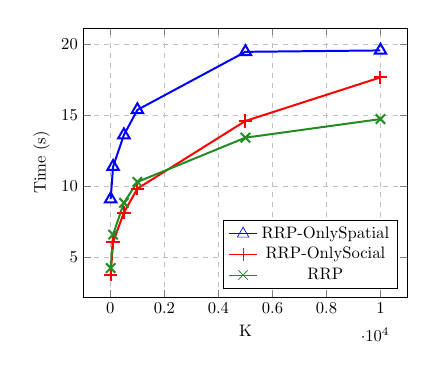
\begin{tikzpicture}[every plot/.append style={very thick}, scale=0.6]
			\begin{axis}[
			    xlabel={K},
			    ylabel={Time (s)},
			    legend pos=south east,
			    xmajorgrids=true,
			    ymajorgrids=true,
			    grid style=dashed,
			   	mark size=4pt
			]
			 
			%\addplot[
			%    color=blue,
			%    mark=x,
			%    ]
			%    coordinates {
			%    (10,73.8)(20,64.22)(40,64.06)(80,64.66)(160,69.06)(320,69.48)(640,64.44)(1280,64.44)
			%    };
			\addplot[
			    color=blue,
			    mark=triangle,
			    ]
			    coordinates {
			    (10, 9.07)(100, 11.36)(500, 13.59)(1000, 15.36)(5000, 19.45)(10000, 19.55)
			    };
			\addplot[
			    color=red,
			    mark=+,
			    ]
			    coordinates {
			    (10, 3.75)(100, 6.04)(500, 8.12)(1000, 9.81)(5000, 14.58)(10000, 17.65)
			    };
			\addplot[
			    color=ForestGreen,
			    mark=x,
			    ]
			    coordinates {
			    (10, 4.21)(100, 6.57)(500, 8.81)(1000, 10.28)(5000, 13.4)(10000, 14.71)
			    };
			%    \legend{DisjointSearch, RRP-OnlySpatial, RRP-OnlySocial, RRP}
			    \legend{RRP-OnlySpatial, RRP-OnlySocial, RRP}
			 
			\end{axis}
		\end{tikzpicture}
		% \caption{Runtime comparison between DisjointSearch and types of RRP algorithms for RZ = 10}
		\caption{Runtime comparison between the types of RRP algorithms for RZ = 25}
		\label{fig:plot-02}
	\end{subfigure}
	\begin{subfigure}[t]{0.33\textwidth}
		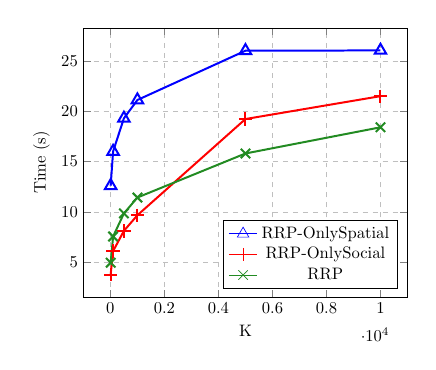
\begin{tikzpicture}[every plot/.append style={very thick}, scale=0.6]
			\begin{axis}[
			    xlabel={K},
			    ylabel={Time (s)},
			    legend pos=south east,
			    xmajorgrids=true,
			    ymajorgrids=true,
			    grid style=dashed,
			    mark size=4pt
			]
			 
			% \addplot[
			%     color=blue,
			%     mark=x,
			%     ]
			%     coordinates {
			%     (10,32.23)(20,29.95)(40,24.9)(80,30.6)(160,24.82)(320,29.76)(640,24.97)(1280,25)
			%     };
			\addplot[
			    color=blue,
			    mark=triangle,
			    ]
			    coordinates {
			    (10, 12.61)(100, 16.01)(500, 19.3)(1000, 21.12)(5000, 26.01)(10000, 26.04)
			    };
			\addplot[
			    color=red,
			    mark=+,
			    ]
			    coordinates {
				(10, 3.79)(100, 6.12)(500, 8.13)(1000, 9.68)(5000, 19.23)(10000, 21.5)
			    };
			\addplot[
			    color=ForestGreen,
			    mark=x,
			    ]
			    coordinates {
			    (10, 4.97)(100, 7.57)(500, 9.86)(1000, 11.44)(5000, 15.81)(10000, 18.41)
			    };
			    % \legend{DisjointSearch, RRP-OnlySpatial, RRP-OnlySocial, RRP}
			    \legend{RRP-OnlySpatial, RRP-OnlySocial, RRP}
			 
			\end{axis}
		\end{tikzpicture}
		% \caption{Runtime comparison between DisjointSearch and types of RRP algorithms for RZ = 1,000}
		\caption{Runtime comparison between the types of RRP algorithms for RZ = 3125}
		\label{fig:plot-03}
	\end{subfigure}
	\begin{subfigure}[t]{0.33\textwidth}
		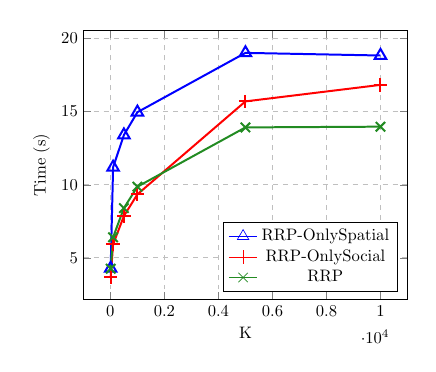
\begin{tikzpicture}[every plot/.append style={very thick}, scale=0.6]
			\begin{axis}[
			    xlabel={K},
			    ylabel={Time (s)},
			    legend pos=south east,
			    xmajorgrids=true,
			    ymajorgrids=true,
			    grid style=dashed,
			    mark size=4pt
			]
			 
			% \addplot[
			%     color=blue,
			%     mark=x,
			%     ]
			%     coordinates {
			%     (10.0, 33.54)(20.0, 25.28)(40.0, 30.72)(80.0, 30.07)(160.0, 29.89)(320.0, 24.95)(640.0, 24.93)(1280.0, 30.34)
			%     };
			\addplot[
			    color=blue,
			    mark=triangle,
			    ]
			    coordinates {
			    (10, 4.27)(100, 11.19)(500, 13.4)(1000, 14.96)(5000, 19.02)(10000, 18.84)
			    % (10, 9.33)(100, 11.81)(500, 13.82)(1000, 15.52)(5000, 19.66)(10000, 19.71) % RZ = 125
			    };
			\addplot[
			    color=red,
			    mark=+,
			    ]
			    coordinates {
			    (10, 3.68)(100, 5.91)(500, 7.86)(1000, 9.34)(5000, 15.7)(10000, 16.83)
			    % (10, 3.83)(100, 6.12)(500, 8.12)(1000, 9.74)(5000, 19.41)(10000, 14.62) % RZ = 125
			    };
			\addplot[
			    color=ForestGreen,
			    mark=x,
			    ]
			    coordinates {
			    (10, 4.25)(100, 6.4)(500, 8.4)(1000, 9.86)(5000, 13.92)(10000, 13.97)
			    % (10, 4.19)(100, 6.56)(500, 8.7)(1000, 10.13)(5000, 14.39)(10000, 19.12) % RZ = 125
			    };
			    % \legend{DisjointSearch, RRP-OnlySpatial, RRP-OnlySocial, RRP}
			    \legend{RRP-OnlySpatial, RRP-OnlySocial, RRP}
			 
			\end{axis}
		\end{tikzpicture}
		% \caption{Runtime comparison between DisjointSearch and types of RRP algorithms for RZ = 100}
		\caption{Runtime comparison between the types of RRP algorithms for RZ = 625}
		\label{fig:plot-03a}
	\end{subfigure}
	\caption{Runtime comparison between the types of RRP algorithms for different resolutions}
\end{figure*}




\begin{figure*}[t]
	\begin{subfigure}[t]{0.5\textwidth}
		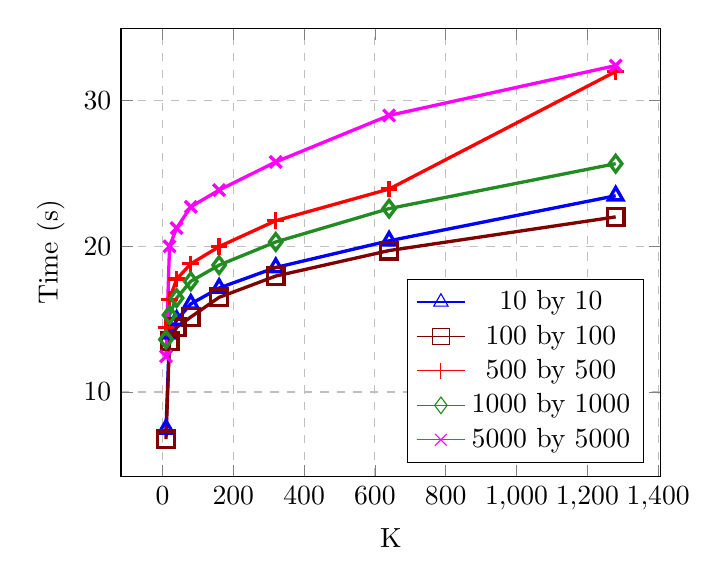
\begin{tikzpicture}[every plot/.append style={very thick}][scale=0.85]
			\begin{axis}[
			    xlabel={K},
			    ylabel={Time (s)},
			    legend pos=south east,
			    xmajorgrids=true,
			    ymajorgrids=true,
			    grid style=dashed,
			    mark size=3pt
			]
			 
			\addplot[
			    color=blue,
			    mark=triangle,
			    ]
			    coordinates {
			    (10.0, 7.45)(20.0, 13.99)(40.0, 14.93)(80.0, 16.04)(160.0, 17.13)(320.0, 18.54)(640.0, 20.37)(1280.0, 23.46)
			    };
			\addplot[
			    color=Maroon,
			    mark=square,
			    ]
			    coordinates {
			    (10.0, 6.76)(20.0, 13.5)(40.0, 14.43)(80.0, 15.14)(160.0, 16.49)(320.0, 17.95)(640.0, 19.7)(1280.0, 22.01)
			    };
			\addplot[
			    color=red,
			    mark=+,
			    ]
			    coordinates {
				(10.0, 14.44)(20.0, 16.36)(40.0, 17.74)(80.0, 18.79)(160.0, 19.97)(320.0, 21.75)(640.0, 23.92)(1280.0, 31.98)
			    };
			\addplot[
			    color=ForestGreen,
			    mark=diamond,
			    ]
			    coordinates {
			    (10.0, 13.6)(20.0, 15.28)(40.0, 16.44)(80.0, 17.59)(160.0, 18.7)(320.0, 20.29)(640.0, 22.58)(1280.0, 25.66)
			    };
			\addplot[
			    color=Magenta,
			    mark=x,
			    ]
			    coordinates {
			    (10.0, 12.44)(20.0, 19.99)(40.0, 21.24)(80.0, 22.7)(160.0, 23.85)(320.0, 25.78)(640.0, 28.97)(1280.0, 32.39)
			    };
			    \legend{10 by 10,100 by 100,500 by 500,1000 by 1000,5000 by 5000}
			 
			\end{axis}
		\end{tikzpicture}
		\caption{Runtime comparison between Resolution and K using only SpatialIndex of RRP}
		\label{fig:plot-07}
	\end{subfigure}
	\begin{subfigure}[t]{0.5\textwidth}
		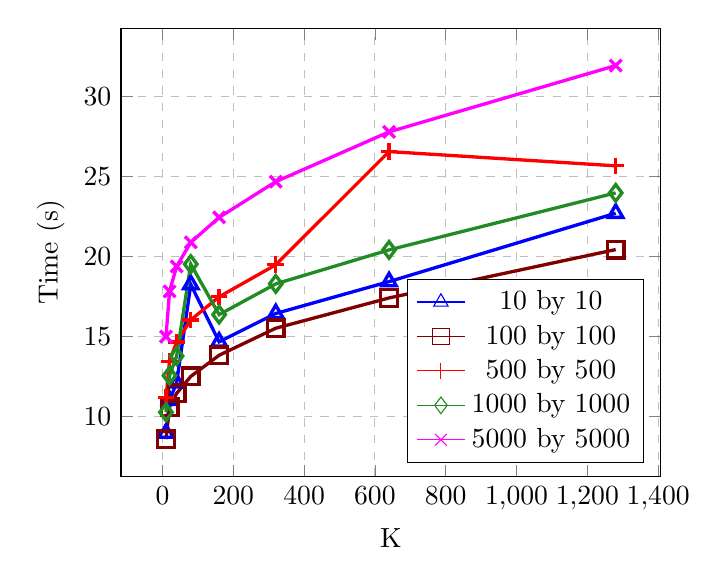
\begin{tikzpicture}[every plot/.append style={very thick}][scale=0.85]
			\begin{axis}[
			    xlabel={K},
			    ylabel={Time (s)},
			    legend pos=south east,
			    xmajorgrids=true,
			    ymajorgrids=true,
			    grid style=dashed,
			    mark size=3pt
			]
			 
			\addplot[
			    color=blue,
			    mark=triangle,
			    ]
			    coordinates {
			    (10.0, 8.98)(20.0, 11.02)(40.0, 12.12)(80.0, 18.26)(160.0, 14.68)(320.0, 16.45)(640.0, 18.44)(1280.0, 22.71)
			    };
			\addplot[
			    color=Maroon,
			    mark=square,
			    ]
			    coordinates {
			    (10.0, 8.6)(20.0, 10.6)(40.0, 11.46)(80.0, 12.52)(160.0, 13.84)(320.0, 15.53)(640.0, 17.42)(1280.0, 20.44)
			    };
			\addplot[
			    color=red,
			    mark=+,
			    ]
			    coordinates {
				(10.0, 11.2)(20.0, 13.47)(40.0, 14.66)(80.0, 16.05)(160.0, 17.49)(320.0, 19.49)(640.0, 26.56)(1280.0, 25.67)
			    };
			\addplot[
			    color=ForestGreen,
			    mark=diamond,
			    ]
			    coordinates {
			    (10.0, 10.28)(20.0, 12.57)(40.0, 13.79)(80.0, 19.53)(160.0, 16.38)(320.0, 18.3)(640.0, 20.42)(1280.0, 23.98)
			    };
			\addplot[
			    color=Magenta,
			    mark=x,
			    ]
			    coordinates {
			    (10.0, 15.01)(20.0, 17.83)(40.0, 19.39)(80.0, 20.89)(160.0, 22.45)(320.0, 24.68)(640.0, 27.79)(1280.0, 31.93)
			    };
			    \legend{10 by 10,100 by 100,500 by 500,1000 by 1000,5000 by 5000}
			 
			\end{axis}
		\end{tikzpicture}
		\caption{Runtime comparison between Resolution and K using both Social+Spatial indices of RRP}
		\label{fig:plot-08}
	\end{subfigure}
	\caption{Runtime comparison between Resolution and K for different types of RRP algorithms}
\end{figure*}